\begin{frame}
	\setbeamercolor{block body}{bg = yellow}
	\begin{block}{}
		\begin{center}
			{\large\textbf{Corso di base JAVA}}\\
			\itshape{Mauro Donadeo}\\
			mail: mauro.donadeo@gmail.com
		\end{center}
	\end{block}
	\setbeamercolor{block body}{bg = white}
	\begin{block}{}	
		\begin{center}
			\large{Le decisioni}\\
			
\includegraphics[width = 30mm]{images/java-logo.jpg}
		\end{center}
	\end{block}	
\end{frame}

\section*{L'enunciato if}
\begin{frame}
\frametitle{Enunciato if}
\begin{block}{}
Il programma \textbf{BankAccount} consente di prelevare tutto il denaro che si vuole
\begin{itemize}
\item il saldo \texttt{balance} può diventare \textbf{\textCl{negativo}}
\begin{itemize}
\item \textbf{balance = balance - amount;}
\end{itemize}
\item \`E una situazione assai poco realistica
\item Quindi il programma deve \textbf{\alert{controllare}} il saldo ed agire di conseguenza. \textit{Consentire il prelievo o no.}
\end{itemize}
\end{block}
\end{frame}

\subsection*{A cosa serve}
\begin{frame}
\begin{columns}
\begin{column}{.5\textwidth}
\begin{block}{}
\textbf{\alert{if (amount $<=$ balance)}}\\
\hfill{\textbf{\textCl{balance = balance - amount;}}}
\end{block}
\begin{block}{}
\begin{itemize}
\item L'enunciato if si usa per realizzare una decisione ed è diviso in due parti
\begin{itemize}
\item una \alert{verifica}
\item un \alert{corpo}
\end{itemize}
\item Il corpo viene eseguito \textbf{\textCl{se e solo se} la verifica ha successo}
\end{itemize}
\end{block}
\end{column}
\begin{column}{.5\textwidth}
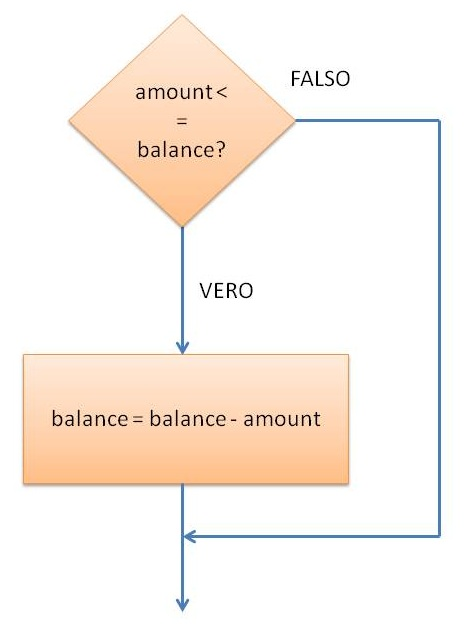
\includegraphics[width = \textwidth]{images/costruttoIf.jpg}
\end{column}
\end{columns}
\end{frame}

\begin{frame}
\frametitle{Tipi di enunciato in Java}
\begin{block}{}
\begin{itemize}
\item Enunciato semplice
\begin{itemize}
\item \textbf{balance = balance - amount;}
\end{itemize}
\item Enunciato composto
\begin{itemize}
\item \textbf{if(x $>=$ 0) x=0;}
\end{itemize}
\item blocco di enunciati
\begin{itemize}
\item \textbf{$\left \{ \mbox{\textbf{\alert{zero o più enunciati di qualsiasi tipo}}} \right \}$}
\end{itemize}
\end{itemize}
\end{block}
\end{frame}
\subsection*{If\ldots then\ldots else\ldots}
\begin{frame}
\begin{block}{}
Proviamo ad emettere un messaggio d'errore in caso di prelievo non consentito:\\
\textbf{if(\alert{amount $<=$ balance})}\\
\hspace{0.7cm}\textbf{balance = balance - amount;}\\
\textbf{if(\alert{amount $>$ balance})} \\
\hspace{0.7cm}\textbf{System.out.println(``Conto scoperto'');} 
\end{block}
\begin{block}{Problema}
Se si modifica la prima verifica, bisogna ricordarsi di modificare anche la seconda.
\end{block}
\begin{block}{Problema}
Se il corpo del primo \texttt{if} viene eseguito, la verifica del secondo \texttt{if} usa il nuovo valore di \texttt{balance},
introducendo \textbf{\textCl{errore logico}}
\begin{itemize}
\item quando si preleva più della metà del saldo disponibile
\end{itemize}
\end{block}
\end{frame}

\begin{frame}
\frametitle{La clausola else}
\begin{block}{}
Per realizzare un'alternativa, si utilizza la clausola \textbf{\textCl{else}} dell'enunciato \texttt{if}\\
\textbf{if(amount $<=$ balance)}\\
\hspace{0.7cm} \textbf{\textCl{balance = balance - amount;}}\\
\textbf{\alert{else}}\\
\hspace{0.7cm}\textbf{\textCl{System.out.println(``Conto aperto'');}}\\
\end{block}
\begin{block}{}
Vantaggio: ora c'è una sola verifica
\begin{itemize}
\item se la verifica ha successo, viene eseguito il primo corpo dell'enunciato \texttt{if/else}
\item altrimenti, viene eseguito il secondo dopo;
\end{itemize}
\end{block}
\end{frame}

\begin{frame}[fragile]
\begin{lstlisting}
if (amount <= balance)
    balance = balance - amount;
else{
    System.out.println("Conto scoperto");
    balance = balance - OVERDRAFT_PENALTY;
}
\end{lstlisting}
\begin{center}
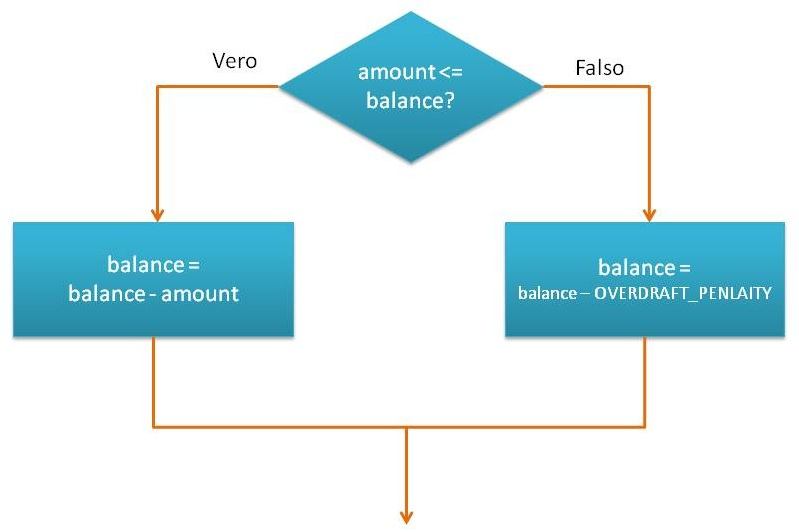
\includegraphics[scale=0.35]{images/costruttoIfElse.jpg}
\end{center}
\end{frame}

\section*{Confronti}
\subsection*{Confronto valori numerici}

\begin{frame}
\begin{block}{}
\begin{huge}
\begin{center}
\textCl{Confrontare valori}
\end{center}
\end{huge}
\end{block}
\end{frame}

\begin{frame}
\begin{block}{}
Le condizioni dell'enunciato if sono molto spesso dei confronti tra due valori\\
\textbf{if(\alert{x $>=$ 0})}\\
Gli operatori di confronto si chiamano operatori relazionali
\end{block}
\begin{block}{}
\centering
\begin{tabular}{|l|l|}
\hline
\textCl{$>$} & Maggiore \\
\hline
\textCl{$>=$} & Maggiore o uguale\\
\hline
\textCl{$<$} & Minore \\
\hline
\textCl{$<=$} & Minore o uguale\\
\hline
\textCl{$==$} & Uguale \\
\hline
\textCl{$!=$} & Diverso\\
\hline
\end{tabular}
\end{block}
\textbf{\alert{Attenzione:}} negli gli operatori da due caratteri \textbf{non} vanno inseriti spazi intermedi 
\end{frame}

\begin{frame}[fragile]
\frametitle{Operatori relazionali}
\begin{block}{}
Fare \textbf{\alert{molta}} attenzione nella differenza tra l'operatore relazionale $==$ e l'operatore assegnazione $=$
\end{block}
\begin{lstlisting}
a = 5; //assegno ad a il valore 5

if(a == 5) //esegue enunciato
   //enunciato
\end{lstlisting}
\end{frame}

\subsection*{Confrontare numeri in virgola mobile}
\begin{frame}
\frametitle{Confrontare numeri in virgola mobile}
\begin{block}{}
I numeri in virgola mobile hanno una precisione limitata ed i calcoli possono introdurre errori di \textCl{arrotondamento} e 
\textCl{troncamento}
\end{block}
\begin{block}{}
Tali errori sono inevitabili e bisogna fare molta attenzione nella formulazione di verifiche che coinvolgono numeri con in 
virgola mobile.
\end{block}
\end{frame}

\begin{frame}
\begin{block}{}
Affinché gli errori di arrotondamento non influenzino la logica del programma, i confronti tra numeri in virgola mobile devono avere
una \textCl{tolleranza}
\end{block}
\begin{block}{}
\begin{itemize}
\item Verifica di uguaglianza tra x ed y (di tipo double): 
\textbf{$$ |x-y| < \epsilon \mbox{ con }\epsilon \mbox{ = 1E-14} $$}
\item Scelta migliore se x,y sono molto grandi o molto piccoli
\textbf{$$|x-y| < \epsilon*max(|x|,|y|) \mbox{ con  }\epsilon \mbox{= 1E-14}$$}
\end{itemize}
\end{block}
\end{frame}

\begin{frame}
\frametitle{Esercizio}
\begin{block}{}
Calcolare la radice quadrata di 2 e confrontare il risultato con 2. Se il risultato è uguale a 2 Stampare ``ok!'' altrimenti ``Errore''
\end{block}
\end{frame}

\subsection*{Confrontare le stringhe}
\begin{frame}
\begin{block}{}
\begin{itemize}
\item Per confrontare stringhe si usa il metodo \textbf{\textCl{equals}}\\
\hspace{0.7cm}\textbf{if(s1.\textbf{\alert{equals(s2)}})}
\item Per confrontare stringhe ignorando la differenza tra maiuscole e minuscole si usa \textbf{\textCl{equalsIgnorecase}}\\
\hspace{0.7cm}\textbf{if(s1.\textbf{\alert{equalsIgnorecase(s2)}})}
\item Non usare \textbf{\alert{mai}} l'operatore di ugualianza per confrontare stringhe. \textbf{\textCl{Usare sempre equals}}
\begin{itemize}
\item Attenzione perché la Virtual Machine \textbf{\alert{NON}} segnalerà alcun errore di sintassi
\end{itemize}
\end{itemize}
\end{block}
\end{frame}

\begin{frame}
\frametitle{Ordinamento lessicografico}
\begin{block}{}
\begin{itemize}
\item Se due stringhe sono diverse, è possibile conoscere la relazione che intercorre tra loro secondo \textbf{\textCl{l'ordinamento 
lessicografico}}, simile al comune ordinamento alfabetico.
\item Il confronto lessicografico tra stringhe si esegue con il metodo \textbf{compareTo}\\
\hspace{0.7cm}\textbf{if(s1.\alert{compareTo}(s2) $<$ 0)}
\item Il metodo compareTo restituisce in valore \texttt{int}
\begin{itemize}
\item \textbf{negativo} se s1 precede s2 nell'ordinamento;
\item \textbf{positivo} se s1 segue s2 nell'ordinamento;
\item \textbf{zero} se s1 e s2 sono identiche.
\end{itemize}
\end{itemize}
\end{block}
\end{frame}

\begin{frame}
\frametitle{Esercizio}
\begin{block}{}
Scrivere un programma che chiede all'utente di inserire tre stringhe (una per riga) visualizza le stringhe in ordine lessicografico 
crescente (una per riga)
\end{block}
\end{frame}
